\documentclass[a5paper,titlepage,10pt,openany]{scrbook}
\usepackage[a5paper,backref]{hyperref}
\usepackage[papersize={148.5mm,215mm},twoside,bindingoffset=0.5cm,hmargin={2cm,2cm},
				vmargin={2cm,2cm},footskip=1.1cm,driver=dvipdfm]{geometry}
\usepackage{palatino}
\usepackage{pstricks}
\usepackage{graphicx}
\usepackage[bahasa]{babel} 
%\usepackage[pdftex]{dropping}
\usepackage{lettrine}
\usepackage{pifont}
\usepackage{enumitem}
\usepackage{wrapfig}
\usepackage{indentfirst}
\usepackage{parcolumns}
\usepackage[titles]{tocloft}
\usepackage{longtable}
%\usepackage[raggedright]{titlesec}
%\usepackage{titletoc}


\renewcommand{\cftchapfont}{%
  \fontsize{9}{8}\selectfont
}

\makeatletter
\renewcommand{\@pnumwidth}{1em} 
\renewcommand{\@tocrmarg}{1em}
\makeatother

\author{Lingkungan St. Petrus Maguwo}
\title{Warta Iman}
\setlength{\parindent}{1cm}
\psset{unit=1mm}

\makeatletter
\renewcommand{\@makeschapterhead}[1]{%
  {\parindent \z@ \centering \normalfont
    \interlinepenalty\@M \Large \bfseries #1\par\nobreak \vskip 20\p@ }}
\renewcommand{\section}{\@startsection {section}{1}{\z@}%
                                   {-3.5ex \@plus -1ex \@minus -.2ex}%
                                   {2.3ex \@plus.2ex}%
%                                   {\normalfont\normalsize\bfseries\centering}}
                                   {\normalfont\normalsize\bfseries}}
\renewcommand\subsection{\@startsection{subsection}{2}{\z@}%
                                     {-3.25ex\@plus -1ex \@minus -.2ex}%
                                     {1.5ex \@plus .2ex}%
                                     {\normalfont\normalsize\bfseries}}
\renewcommand\subsubsection{\@startsection{subsubsection}{3}{\parindent}%
                                    {3.25ex \@plus1ex \@minus.2ex}%
                                    {-1em}%
                                    {\normalfont\normalsize\bfseries}}

\makeatother

\makeatletter  % Allow the use of @ in command names
\long\def\@makecaption#1#2{%
  \vskip\abovecaptionskip
  \sbox\@tempboxa{{#1#2}}%
  \ifdim \wd\@tempboxa >\hsize
    {#1#2\par}
  \else
    \hbox to\hsize{\hfil\box\@tempboxa\hfil}%
  \fi
  \vskip\belowcaptionskip}
\makeatother   % Cancel the effect of \makeatletter

\newcommand{\chap}[1]{%
    \chapter*{#1}
	\addcontentsline{toc}{chapter}{#1}
    }

\newcommand{\sumber}[1]{%    
	\begin{flushright}
	{\emph{#1}}
	\end{flushright}
}
\newcommand{\qti}[1]{%    
	\begin{quote}
	{\emph{#1}}
	\end{quote}
}

\hyphenation{sa-u-da-ra-ku}
\hyphenation{ke-ri-ngat}
\hyphenation{je-ri-tan}
\hyphenation{hu-bung-an}
\hyphenation{me-nya-dari}
\hyphenation{Eng-kau}
\hyphenation{ke-sa-lah-an}
\hyphenation{ba-gai-ma-na}
\hyphenation{Tu-han}
\hyphenation{di-per-ca-ya-kan}
\hyphenation{men-ja-uh-kan}
\hyphenation{bu-kan-lah}
\hyphenation{per-sa-tu-kan-lah}
\hyphenation{ma-khluk}
\hyphenation{Sem-buh-kan-lah}
\hyphenation{ja-lan}
\hyphenation{mem-bu-tuh-kan}
\hyphenation{be-ri-kan-lah}
\hyphenation{me-ra-sa-kan}
\hyphenation{te-man-ilah}
\hyphenation{mem-bi-ngung-kan}
\hyphenation{di-ka-gum-i}
\hyphenation{ta-ngis-an-Mu}
\hyphenation{mi-lik-ilah}

\renewcommand{\figurename}{~}
\renewcommand\thefigure{~}

\setlist{noitemsep}
\renewcommand{\thesection}{\Alph{section}}

\begin{document}
\thispagestyle{empty}
\thispagestyle{empty}
\newcommand{\edisi}[1]{%
\DeclareFixedFont{\PT}{T1}{ppl}{b}{}{0.7in}
\DeclareFixedFont{\PTit}{T1}{ppl}{b}{it}{0.7in}
\DeclareFixedFont{\PTsmall}{T1}{ppl}{b}{it}{0.25in}
\DeclareFixedFont{\PTsmaller}{T1}{ppl}{b}{it}{0.175in}
\DeclareFixedFont{\PTsmallest}{T1}{ppl}{b}{it}{0.15in}

\begin{pspicture}(14cm,2cm)
\rput[rb](10.35cm,3cm){\PTsmallest {#1}}
\rput[lb](-2cm,1.5cm){\PT {WARTA IMAN}}
\rput[lb](0cm,0.5cm){\PTsmall {Lingkungan St. Petrus Maguwo}}
\end{pspicture}%
}

\newcounter{kgkcounter}[chapter]
\renewcommand{\thekgkcounter}{\arabic{kgkcounter}. }
\newcommand{\kgk}[1]{\refstepcounter{kgkcounter}\textbf{\flushleft \textbf{\thekgkcounter #1}}\\}

\newcommand{\kutipan}[1]{%
\noindent{\framebox{\parbox{10cm}{\centering\emph{#1}}}}}

\edisi{November 2011}

%\vspace{1cm}

\begin{center}
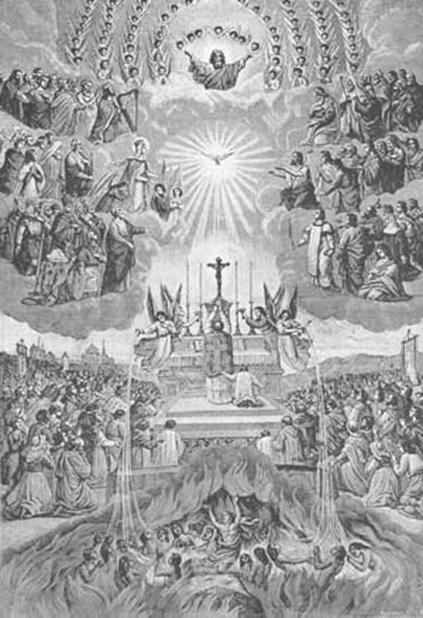
\includegraphics[scale=0.85]{gambar/purgatory2.jpg}
\end{center}

%\vspace{1cm}

\begin{center}
{\PTsmaller {Kasih, kerendahan hati, dan menurut pada kehendak Allah }}
\end{center}

\setlength{\parindent}{1cm}
\pagestyle{plain}
\chap{Mengapa kita berpantang dan berpuasa?}

\section*{Kamu mau pantang apa dalam Masa Prapaska ini?}
Ya, seharusnya pertanyaan ini timbul di hati kita sebelum kita memulai masa Prapaska, jika kita ingin membuat Masa Prapaska ini suatu kesempatan kita untuk bertumbuh secara rohani. Inilah kesempatan bagi kita untuk merenungkan, hal apa yang paling kita sukai, yang dapat kita `korbankan' demi menyatakan kasih kepada Tuhan, yang lebih dahulu mengasihi kita. Hal yang disukai bisa berbeda antara orang yang satu dengan yang lain, dan karena itu, yang paling dapat merasakan efeknya adalah orang yang bersangkutan. Ada keluarga teman saya yang senengnya menonton TV, kemudian mereka memutuskan untuk mengurangi nonton TV sehingga hanya 1 kali seminggu, hari Sabtu. Waktu yang tadinya dipakai untuk nonton TV dipergunakan untuk berkumpul dan berdoa bersama. Tahun lalu, di samping pantang daging,  suami saya memilih pantang kopi, dan saya pantang sambal. Minggu pertama sangat berat buat suami saya, yang sudah bertahun-tahun terbiasa minum kopi minimal 3 gelas sehari. Awalnya, kepalanya pusing dan selalu mengantuk, namun toh akhirnya bisa juga. Lalu saya, dengan pantang sambal maka makan apapun rasanya kurang pas di lidah saya. Tapi hal ini mengajarkan saya supaya tidak lekas komplain. Sebab ini bukan apa-apa jika dibandingkan dengan pengorbanan Yesus di kayu salib.

Memang, kita dapat menemukan banyak jenis pantang, dan mungkin pula kita dapat memilih yang  sedikit lebih sulit, yang melibatkan penguasaan diri. Contohnya, pantang membicarakan kekurangan orang lain, pantang membicarakan kelebihan diri sendiri,  pantang mengeluh/ komplain, pantang berprasangka negatif atau pantang marah bagi orang yang lekas emosi. Selanjutnya kita diajak untuk lebih mengarahkan hati kepada Tuhan dan berusaha menyenangkan hati-Nya dengan pikiran dan perbuatan kita.  Ini adalah contoh yang paling sederhana dari ucapan, ``Aku mau mati terhadap diri sendiri dan hidup bagi Tuhan'' (lih. Rom 6:8). Jadi pantang dan puasa bukan sekedar tidak makan daging atau tidak jajan, tetapi selebihnya tak ada yang berubah dalam hubungan kita dengan Tuhan. Kita diundang untuk melihat ke dalam diri kita, untuk melihat kebiasaan apakah yang selama ini menghalangi kita untuk lebih dekat kepada Tuhan. Mari, pada masa Prapaska ini, kita membuat suatu usaha nyata untuk mengambil `penghalang' tersebut dalam hidup kita. Dan dengan demikian, kita dapat mengalami hubungan yang lebih baik dengan Tuhan.

\section*{Buat apa berpantang dan berpuasa}
Setiap masa Prapaska, kita diajak oleh Gereja untuk bersama-sama berpantang dan berpuasa. Puasa dan pantang yang disyaratkan oleh Gereja Katolik sebenarnya tidak berat, sehingga sesungguhnya tidak ada alasan bagi kita untuk tidak melakukannya. Namun, meskipun kita melakukannya, tahukah kita arti pantang dan puasa tersebut bagi kita umat Katolik?

Bagi kita orang Katolik, puasa dan pantang artinya adalah tanda pertobatan, tanda penyangkalan diri, dan tanda kita mempersatukan sedikit pengorbanan kita dengan pengorbanan Yesus di kayu salib sebagai silih dosa kita dan demi mendoakan keselamatan dunia. Jika pantang dan puasa dilakukan dengan hati tulus maka keduanya dapat menghantar kita bertumbuh dalam kekudusan. Kekudusan ini yang dapat berbicara lebih lantang dari pada khotbah yang berapi-api sekalipun, dan dengan kekudusan inilah kita mengambil bagian dalam karya keselamatan Allah. Allah begitu mengasihi dan menghargai kita, sehingga kita diajak oleh-Nya untuk mengambil bagian dalam karya keselamatan ini. Caranya, dengan bertobat, berdoa dan melakukan perbuatan kasih, dan sesungguhnya inilah yang bersama-sama kita lakukan dalam kesatuan dengan Gereja pada masa Prapaska.

Jangan kita lupa bahwa  masa puasa selama 40 hari ini adalah karena mengikuti teladan Yesus, yang juga berpuasa selama 40 hari 40 malam, sebelum memulai tugas karya penyelamatan-Nya (lih. Mat 4: 1-11; Luk 4:1-13). Yesus berpuasa di padang gurun dan pada saat berpuasa itu Ia digoda oleh Iblis. Yesus mengalahkan godaan tersebut dengan bersandar pada Sabda Tuhan yang tertulis dalam Kitab Suci. Maka, kitapun hendaknya bersandar pada Sabda Tuhan untuk mengalahkan godaan pada saat kita berpuasa. Dengan doa dan merenungkan Sabda Tuhan, kita akan semakin menghayati makna puasa dan pantang pada Masa Prapaska ini.

\section*{Puasa dan pantang tak terlepas dari doa}
Jadi puasa dan pantang bagi kita tak pernah terlepas dari doa. Dalam masa Prapaska, puasa, pantang dan doa disertai juga dengan perbuatan amal kasih bersama-sama dengan anggota Gereja yang lain. Dengan demikian, pantang dan puasa bagi kita orang Katolik merupakan latihan rohani yang mendekatkan diri pada Tuhan dan sesama, dan bukan untuk hal lain, seperti semata-mata `menyiksa badan', diet/ supaya kurus, menghemat, dll. Janganlah kita lupa, tujuan utama puasa dan pantang adalah supaya kita dapat lebih menghayati kasih Tuhan yang kita terima dan kasih kepada Tuhan. Kita diajak untuk merenungkan sengsara Kristus demi menyelamatkan kita, dan selanjutnya kita diajak untuk menyatakan kasih kita kepada Kristus, dengan mendekatkan diri kepada-Nya dan sesama.

\section*{Dengan puasa kita mengambil bagian dalam karya keselamatan Allah}

Dengan mendekatkan dan menyatukan diri dengan Tuhan, maka kehendak-Nya menjadi kehendak kita. Dan karena kehendak Tuhan yang terutama adalah keselamatan dunia, maka melalui puasa dan pantang, kita diundang Tuhan untuk mengambil bagian dalam karya penyelamatan dunia, yaitu dengan berdoa dan menyatukan pengorbanan kita dengan pengorbanan Yesus di kayu salib. Kita pun dapat mendoakan keselamatan dunia dengan mulai mendoakan bagi keselamatan orang-orang yang terdekat dengan kita: orang tua, suami/ istri, anak-anak, saudara, teman, dan juga kepada para imam dan pemimpin Gereja. Kemudian kita dapat pula berdoa bagi para pemimpin negara, para umat beriman, ataupun mereka yang belum mengenal Kristus.

\section*{Puasa dan Pantang menurut Ketentuan Gereja Katolik}

Berikut ini mari kita lihat ketentuan tobat dengan puasa dan pantang, menurut Kitab Hukum Gereja Katolik:
\begin{enumerate}
\item \textbf{Kan. 1249}:  Semua orang beriman kristiani wajib menurut cara masing-masing melakukan tobat demi hukum ilahi; tetapi agar mereka semua bersatu dalam suatu pelaksanaan tobat bersama, ditentukan hari-hari tobat, dimana umat beriman kristiani secara khusus meluangkan waktu untuk doa, menjalankan karya kesalehan dan amal-kasih, menyangkal diri sendiri dengan melaksanakan kewajiban-kewajibannya secara lebih setia dan terutama dengan berpuasa dan berpantang, menurut norma kanon-kanon berikut.

\item \textbf{Kan. 1250}: Hari dan waktu tobat dalam seluruh Gereja ialah setiap hari Jumat sepanjang tahun, dan juga masa prapaskah.

\item \textbf{Kan. 1251}: Pantang makan daging atau makanan lain menurut ketentuan Konferensi para Uskup hendaknya dilakukan setiap hari Jumat sepanjang tahun, kecuali hari Jumat itu kebetulan jatuh pada salah satu hari yang terhitung hari raya; sedangkan pantang dan puasa hendaknya dilakukan pada hari Rabu Abu dan pada hari Jumat Agung, memperingati Sengsara dan Wafat Tuhan Kita Yesus Kristus.

\item \textbf{Kan. 1252}: Peraturan pantang mengikat mereka yang telah berumur genap empat belas tahun; sedangkan peraturan puasa mengikat semua yang berusia dewasa sampai awal tahun ke enampuluh; namun para gembala jiwa dan orangtua hendaknya berusaha agar juga mereka, yang karena usianya masih kurang tidak terikat wajib puasa dan pantang, dibina ke arah cita-rasa tobat yang sejati.

\item \textbf{Kan. 1253}: Konferensi para Uskup dapat menentukan dengan lebih rinci pelaksanaan puasa dan pantang; dan juga dapat mengganti-kan seluruhnya atau sebagian wajib puasa dan pantang itu dengan bentuk-bentuk tobat lain, terutama dengan karya amal-kasih serta latihan-latihan rohani.
\end{enumerate}

Memang sesuai dari yang kita ketahui, ketentuan dari Konferensi para Uskup di Indonesia menetapkan selanjutnya:

\begin{enumerate}
\item Hari Puasa dilangsungkan pada hari Rabu Abu dan Jumat Agung. Hari Pantang dilangsungkan pada hari Rabu Abu dan tujuh Jumat selama Masa Prapaska sampai dengan Jumat Agung.

\item Yang wajib berpuasa ialah semua orang Katolik yang berusia 18 tahun sampai awal tahun ke-60. Yang wajib berpantang ialah semua orang Katolik yang berusia genap 14 tahun ke atas.

\item Puasa (dalam arti yuridis) berarti makan kenyang hanya sekali sehari. Pantang (dalam arti yuridis) berarti memilih pantang daging, atau ikan atau garam, atau jajan atau rokok. Bila dikehendaki masih bisa menambah sendiri puasa dan pantang secara pribadi, tanpa dibebani dengan dosa bila melanggarnya.
\end{enumerate}

\noindent{Maka penerapannya adalah sebagai berikut:}
\small
\begin{enumerate}
\item Kita berpantang setiap hari Jumat sepanjang tahun (contoh: pantang daging, pantang rokok dll) kecuali jika hari Jumat itu jatuh pada hari raya, seperti dalam oktaf masa Natal dan oktaf masa Paskah. Penetapan pantang setiap Jumat ini adalah karena Gereja menentukan hari Jumat sepanjang tahun (kecuali yang jatuh di hari raya) adalah hari tobat. Namun, jika kita mau melakukan yang lebih, silakan berpantang, setiap hari selama Masa Prapaska.

\item Jika kita berpantang, pilihlah makanan/ minuman yang paling kita sukai. Pantang daging adalah contohnya, atau yang lebih sukar mungkin pantang garam. Tapi ini bisa juga berarti pantang minum kopi bagi orang yang suka sekali kopi, dan pantang sambal bagi mereka yang sangat suka sambal, pantang rokok bagi mereka yang merokok, pantang jajan bagi mereka yang suka jajan. Jadi jika kita pada dasarnya tidak suka jajan, jangan memilih pantang jajan, sebab itu tidak ada artinya.

\item Pantang tidak terbatas hanya makanan, namun pantang makanan dapat dianggap sebagai hal yang paling mendasar dan dapat dilakukan oleh semua orang. Namun jika satu dan lain hal tidak dapat dilakukan, terdapat pilihan lain, seperti pantang kebiasaan yang paling mengikat, seperti pantang nonton TV, pantang 'shopping', pantang ke bioskop, pantang `gossip', pantang main `game', pantang buka Internet, dll. Jika memungkinkan tentu kita dapat melakukan gabungan antara pantang makanan/ minuman dan pantang kebiasaan ini.

\item Puasa minimal dalam setahun adalah Hari Rabu Abu dan Jumat Agung, namun bagi yang dapat melakukan lebih, silakan juga berpuasa dalam ketujuh hari Jumat dalam masa Prapaska, (atau bahkan setiap hari dalam masa Prapaska).

\item Waktu berpuasa, kita makan kenyang satu kali, dapat dipilih sendiri pagi, siang atau malam. Harap dibedakan makan kenyang dengan makan sekenyang-kenyangnya. Karena maksud berpantang juga adalah untuk melatih pengendalian diri, maka jika kita berbuka puasa/ pada saat makan kenyang, kita juga tetap makan seperti biasa, tidak berlebihan. Juga makan kenyang satu kali sehari bukan berarti kita boleh makan snack/ cemilan berkali-kali sehari. Ingatlah tolok ukurnya adalah pengendalian diri dan keinginan untuk turut merasakan sedikit penderitaan Yesus, dan mempersatukan pengorbanan kita dengan pengorbanan Yesus di kayu salib demi keselamatan dunia.

\item Maka pada saat kita berpuasa, kita dapat mendoakan untuk pertobatan seseorang, atau mohon pengampunan atas dosa kita. D oa-doa seperti inilah yang sebaiknya mendahului puasa, kita ucapkan di tengah-tengah kita berpuasa, terutama saat kita merasa haus/ lapar, dan doa ini pula yang menutup puasa kita/ sesaat sebelum kita makan. Di sela-sela kesibukan sehari-hari kita dapat mengucapkan doa sederhana, ``Ampunilah aku, ya Tuhan. Aku mengasihi-Mu, Tuhan Yesus. Mohon selamatkanlah \ldots.'' (sebutkan nama orang yang kita kasihi)

\item Karena yang ditetapkan di sini adalah syarat minimal, maka kita sendiri boleh menambahkannya sesuai dengan kekuatan kita. Jadi boleh saja kita berpuasa dari pagi sampai siang, atau sampai sore, atau bagi yang memang dapat melakukannya, sampai satu hari penuh. Juga tidak menjadi masalah, puasa sama sekali tidak makan dan minum atau minum sedikit air. Diperlukan kebijaksanaan sendiri (prudence) untuk memutuskan hal ini, yaitu seberapa banyak kita mau menyatakan kasih kita kepada Yesus dengan berpuasa, dan seberapa jauh itu memungkinkan dengan kondisi tubuh kita. Walaupun tentu, jika kita terlalu banyak `excuse' ya berarti kita perlu mempertanyakan kembali, sejauh mana kita mengasihi Yesus dan mau sedikit berkorban demi mendoakan keselamatan dunia.
\end{enumerate}
\normalsize
\section*{Tidak terbatas Pantang dan Puasa dan derma/amal}

Dalam masa Prapaska ini, dapat pula kita melakukan sesuatu yang baik yang belum secara konsisten kita lakukan. Misal, bangun lebih pagi setiap hari untuk berdoa, misal dari yang biasanya 5 menit, usahakan jadi 10 menit; atau dari yang biasanya 10 menit, usahakan jadi 20 menit, atau yang 30 menit jadi 1 jam. Memulai hari dengan berdoa dan merenungkan Sabda Tuhan adalah sesuatu yang perlu kita usahakan setiap hari.

Mengikuti Misa Harian (di samping Misa hari Minggu, tentu saja) adalah sesuatu yang dapat pula kita lakukan, jika itu memang memungkinkan dalam situasi kita. Jangan terlalu cepat mengatakan tidak mungkin, jika belum pernah mencoba. Apalagi jika kita tidak mencobanya karena malas bangun pagi. Mengikuti Misa dan menyambut Kristus dalam Ekaristi adalah bukti yang nyata bahwa kita sungguh menghargai apa yang telah dilakukan-Nya bagi kita di kayu salib demi keselamatan kita. Kita dapat pula meluangkan waktu untuk doa Adorasi, di hadapan Sakramen Maha Kudus, jika memang ada kapel Adorasi di paroki/ di kota tempat kita tinggal. Atau kita dapat mulai berdoa Rosario setiap hari. Atau mulai dengan setia meluangkan waktu untuk mempelajari Kitab Suci dan Katekismus Gereja Katolik. Atau mengikuti Ibadat Jalan Salib di gereja, atau jika tidak mungkin, melakukannya bersama dengan keluarga di rumah.

Dalam relasi kita dengan sesama, juga tidak terbatas dengan `asal sudah nyumbang, maka sudah beres'. Dengan merenungkan sengsara Tuhan Yesus, maka kita diajak untuk lebih peka terhadap sikap kita terhadap sesama yang kurang beruntung. Misalnya, yang paling dekat adalah pembantu rumah tangga dan supir. Pernahkah kita memberi kesempatan pada mereka untuk beristirahat, misalnya memberi mereka libur? Libur di sini tidak termasuk hanya pada libur Lebaran, dst, tetapi libur/ istirahat agar mereka juga dapat berekreasi dan melepas lelah. Atau apakah kita menjalin persahabatan dengan sesama anggota Paroki yang berkekurangan?

Wah, banyak sekali sesungguhnya yang dapat kita lakukan, jika kita sungguh ingin bertumbuh di dalam iman. Namun seungguhnya, mulailah saja dengan langkah kecil dan sederhana. St. Theresia dari Liseux pernah mengatakan tipsnya, yaitu, ``Lakukanlah perbuatan-perbuatan yang kecil dan sederhana, namun dengan kasih yang besar.''

\section*{Penutup}

Maka untuk menjawab pertanyaan awal, ``Mau pantang apa aku pada Masa Prapaska ini?'', kita perlu kembali melihat ke dalam hati kita masing-masing. Pasti jika kita mau jujur, akan selalu ada yang dapat kita lakukan. Mengurangi nonton TV, mengurangi ngemil/ jajan, mengurangi nonton bioskop, tidak main game di internet, dll hanya contoh saja, namun itu belum lengkap, jika kita tidak menggunakan waktu tersebut, untuk hal-hal lain yang lebih mendukung perbuatan kasih kita kepada Tuhan dan sesama.

Ya, dengan Rabu Abu, kita diingatkan bahwa hidup kita di dunia ini hanyalah sementara, maka mari kita mempersiapkan diri bagi kehidupan kita yang sesungguhnya di surga kelak. Kita hanya dapat masuk surga dan memandang Tuhan hanya jika kita memiliki kekudusan itu (lih. Ibr 12:14), maka sudah saatnya kita bertanya pada diri sendiri: sudahkah aku hidup kudus? Masa pertobatan adalah masa rahmat yang Tuhan berikan pada kita, untuk mengatur kembali fokus kehidupan kita. Apakah yang menjadi pusat kegiatanku sehari-hari: aku atau Tuhan? Jika kita masih banyak menemukan `aku' sebagai pusatnya, mungkin sudah saatnya kita mulai mengubahnya \ldots

\sumber{Ingrid Listiati\\http://www.katolisitas.org}

\chap{Pesan Bapa Suci Benektus XVI
untuk Masa Prapaskah 2012}

``Dan  marilah kita saling memperhatikan supaya kita saling mendorong dalam kasih dan dalam pekerjaan baik'' (Ibr 10:24).

\small
Saudara dan saudari yang terkasih,

Masa Prapaskah sekali lagi memberikan kepada kita sebuah kesempatan untuk merenungkan inti terdalam dari kehidupan seorang Kristen, yaitu: perbuatan amal kasih. Ini adalah waktu yang tepat untuk memperbaharui perjalanan iman kita, baik sebagai seorang individu maupun sebagai bagian dari komunitas, dengan bimbingan Sabda Tuhan dan sakramen-sakramen Gereja. Perjalanan ini adalah perjalanan yang ditandai dengan doa dan berbagi, hening dan berpuasa, sebagai antisipasi menyambut sukacita Paskah.

Tahun ini saya ingin mengajukan beberapa pemikiran dalam terang ayat-ayat Kitab Suci yang diambil dari Surat kepada umat Ibrani: ``Dan marilah kita kita saling memperhatikan supaya kita saling mendorong dalam kasih dan dalam pekerjaan baik''. Kata-kata ini adalah bagian dari perikop di mana sang penulis surat yang kudus menghimbau kita untuk menaruh kepercayaan di dalam Yesus Kristus sebagai Imam Agung yang telah memenangkan pengampunan Allah bagi kita dan membuka jalan kepada Tuhan. Mengimani Kristus membuat kita mampu menghasilkan buah di dalam hidup yang ditopang oleh tiga kebaijkan teologis: hal itu berarti menghampiri Tuhan ``dengan hati tulus dan penuh iman'' (ay.22), tetap ``teguh dalam harapan yang kita nyatakan'' (ay.23) dan senantiasa berusaha untuk menjalani hidup yang dibangun di atas ``cinta kasih dan pekerjaan-pekerjaan baik'' (ay.24), bersama dengan saudara dan saudari kita. Sang penulis surat tersebut menyatakan bahwa untuk mempertahankan hidup yang dibentuk oleh Injil, adalah penting untuk berpartisipasi secara aktif dalam liturgi dan doa bersama komunitas, dengan mengingat akan tujuan eskatologis untuk bersatu secara penuh dengan Tuhan (ay.25). Di sini saya ingin membuat refleksi atas ayat 24, yang memberikan pengajaran yang ringkas, bernilai, dan tepat di segala zaman, atas tiga aspek hidup Kristiani, yaitu: kepedulian kepada sesama, kasih timbal balik, dan kekudusan pribadi.

\section{``Dan  marilah kita saling memperhatikan..'' : tanggung jawab terhadap para saudara dan saudari kita.}

Aspek pertama adalah sebuah undangan untuk ``peduli'' : kata kerja bahasa Yunani yang dipakai di sini adalah katanoein, yang artinya adalah untuk memeriksa (menyelidiki), untuk menaruh perhatian, untuk mengamati dengan seksama dan percaya akan sesuatu. Kita menjumpai kata ini di dalam Injil ketika Yesus mengundang para murid untuk ``memperhatikan'' burung-burung gagak, yang tanpa bekerja keras, berada di tengah perhatian dan pemeliharaan Penyelenggaraan Ilahi (bdk. Luk 12:24) dan untuk ``memeriksa'' balok di dalam mata kita sendiri sebelum mengeluarkan selumbar dari mata saudara kita (bdk. Luk 6:41). Di dalam ayat yang lain dari Surat kepada orang-orang Ibrani, kita menemukan ajakan untuk ``mengarahkan pikiranmu kepada Yesus'' (3:1), Rasul dan Imam Besar dari iman kita. Maka kata kerja yang mengantar pengajaran kita mengatakan kepada kita untuk memperhatikan sesama, pertama-tama kepada Yesus, untuk saling memperhatikan satu sama lain, dan tidak tinggal dalam keterasingan serta sikap acuh tak acuh kepada keadaan sesama kita. Namun demikian, terlalu sering sikap yang kita tunjukkan justru sebaliknya: yaitu pengabaian dan keacuhan yang lahir dari keegoisan yang disamarkan sebagai tindakan menghargai ``privasi''. Saat ini pun, suara Tuhan meminta kita semua untuk saling memperhatikan satu sama lain. Bahkan hari ini, Tuhan meminta kita untuk menjadi ``penjaga'' saudara dan saudari kita (Kej 4:9), untuk membangun suatu relasi yang didasarkan atas kepedulian satu sama lain dan perhatian kepada kesejahteraan integral jasmani dan rohani dari sesama kita. Perintah yang utama untuk mengasihi satu sama lain menuntut kita untuk mengenali tanggung jawab kita kepada sesama yang, sebagaimana halnya kita sendiri, adalah ciptaan dan anak-anak Tuhan sendiri. Menjadi saudara dan saudari dalam kemanusiaan dan, dalam banyak hal,  juga dalam iman, selayaknya menolong kita untuk mengenali di dalam diri sesama kita, sebuah kebalikan dari diri kita (alter ego), yang dicintai tanpa batas oleh Tuhan. Jika kita menanamkan pada diri kita cara ini yang memandang sesama sebagai saudara dan saudari kita, maka solidaritas, keadilan, belas kasihan dan bela rasa akan secara alamiah berkembang di dalam hati kita. Sang Pelayan Tuhan Paus Paulus VI pernah menyatakan bahwa dunia saat ini menderita terutama karena kurangnya persaudaraan: ``Kebudayaan umat manusia sedang sangat sakit. Penyebabnya bukanlah karena berkurangnya sumber-sumber daya alam, dan bukan juga karena kontrol monopoli dari segelintir orang: melainkan lebih karena melemahnya ikatan persaudaraan di antara pribadi-pribadi dan di antara bangsa-bangsa (Populorum Progressio, 66).

Kepedulian kepada sesama berkaitan juga dengan menginginkan segala yang baik untuk mereka dari setiap sudut pandang: baik fisik, moral, maupun spiritual. Budaya kontemporer nampaknya telah kehilangan naluri untuk membedakan yang baik dari yang jahat, namun disadari tetap ada suatu kebutuhan yang nyata untuk menyatakan kembali bahwa kebaikan itu ada dan akan mengatasi [yang jahat], karena Allah ``baik dan berbuat baik'' (Mzm 119:68). Kebaikan adalah segala sesuatu yang bersifat memberi, melindungi, dan menjunjung tinggi kehidupan, persaudaraan, dan persekututuan. Maka tanggung jawab kepada sesama berarti menginginkan dan mengusahakan kebaikan sesama, dalam harapan bahwa mereka pun menjadi mudah menerima kebaikan dan tuntutan- tuntutannya. Peduli kepada sesama berarti menjadi peka akan kebutuhan-kebutuhan mereka. Injil Suci memperingatkan kita akan bahaya bahwa hati kita dapat menjadi keras karena ``ketidaksadaran spiritual'', yang membuat kita tidak peka dan mati rasa terhadap penderitaan sesama. Penulis Injil Lukas mengaitkan dua perumpaan Yesus dengan membuat contoh. Di dalam perumpamaan tentang Orang Samaria yang Baik Hati, sang imam dan sang orang Lewi lewat begitu saja,  tidak peduli akan keberadaan seseorang yang dirampok dan dipukuli oleh para perampok (bdk. Luk 10:30-32). Dalam kisah perumpamaan Orang Kaya dan Lazarus yang Miskin, si orang kaya tidak peduli pada kemiskinan Lazarus, yang sedang kelaparan hingga sekarat di depan pintu rumahnya yang ada di depan matanya (bdk. Luk 16:19). Kedua perumpamaan tersebut menunjukkan contoh-contoh kebalikan dari  ``menjadi peduli'', yaitu sikap menaruh perhatian kepada sesama dengan penuh cinta dan belas kasihan. Apa yang menghalangi pandangan kemanusiaan dan penuh cinta kepada saudara dan saudari kita ini? Seringkali, penyebabnya adalah kepemilikan kekayaan materi dan perasaan berkecukupan akan segala sesuatu, namun bisa juga penyebabnya adalah kecenderungan untuk meletakkan segala kepentingan/ keinginan, dan masalah kita sendiri di atas semua yang lain. Kita tak pernah boleh gagal untuk ``menunjukkan belas kasihan'' kepada mereka yang menderita. Hati kita tak pernah boleh terlalu terbungkus rapat oleh urusan-urusan dan masalah-masalah kita sehingga hati kita tak mampu mendengar jeritan kaum miskin. Kerendahan hati dan pengalaman pribadi akan penderitaan dapat membangkitkan dalam diri kita, suatu naluri belas kasihan dan empati. ``Orang benar mengetahui hak orang lemah, tetapi orang fasik tidak memahaminya'' (Ams 29:7). Kita kemudian dapat memahami sikap dari ``mereka yang meratap'' (Mat 5:5), mereka yang mampu melihat melampaui diri sendiri dan merasakan belas kasihan terhadap penderitaan orang lain. Menjangkau orang lain dan membuka hati kita kepada kebutuhan-kebutuhan mereka dapat menjadi sebuah kesempatan bagi  keselamatan dan keadaan terberkati.

``Menjadi peduli satu sama lain'' juga mengikutsertakan sikap menaruh perhatian pada kesejahteraan jasmani dan rohani satu sama lain. Di sini saya ingin menyebutkan sebuah aspek hidup Kristiani, yang saya percaya telah cukup terlupakan selama ini: koreksi persaudaraan dalam pandangan keselamatan abadi. Dewasa ini, secara umum, kita menjadi sangat peka kepada gagasan perbuatan amal kasih dan kepedulian kepada kesejahteraan fisik dan materi dari sesama, namun hampir sepenuhnya diam mengenai tanggung jawab spiritual kita kepada saudara dan saudari kita. Hal ini tidak menjadi persoalan di dalam jemaat Gereja perdana atau di dalam komunitas yang telah sangat dewasa dalam iman, [yaitu] mereka yang peduli tidak hanya terhadap kesehatan fisik sesama mereka, tetapi juga terhadap kesehatan spiritual dan kehidupan kekal mereka. Kitab Suci berkata kepada kita: ``Janganlah mengecam seorang pencemooh, supaya engkau jangan dibencinya, kecamlah orang bijak, maka engkau akan dikasihinya'' (Ams 9:8). Kristus sendiri memerintahkan kita untuk menasehati saudara kita yang berbuat dosa (bdk. Mat 18:15). Kata yang dipergunakan untuk mengekpresikan koreksi persaudaraan – elenchein – adalah sama seperti yang biasa digunakan untuk menunjukkan misi kenabian dari orang-orang Kristen untuk menentang generasi yang mengikuti kejahatan (bdk. Ef 5:11). Tradisi Gereja juga memasukkan ``memberi nasehat kepada para pendosa'' di antara karya-karya karitatif rohani (belas kasihan secara rohani). Adalah penting untuk mengembalikan dimensi ini dari perbuatan amal kasih Kristiani. Kita tidak boleh tinggal diam dalam menghadapi kejahatan. Saya berpikir tentang semua umat Kristen itu yang,  karena pertimbangan manusiawi atau semata-mata karena pertimbangan kenyamanan pribadi, memilih berkompromi dengan mentalitas yang umum, daripada mengingatkan saudara dan saudarinya terhadap cara berpikir dan bertindak yang bertentangan dengan kebenaran dan yang tidak mengikuti jalan kebaikan. Menasehati secara Kristiani, tidak pernah dimotivasi oleh semangat menuduh atau menuntut balas, melainkan selalu digerakkan oleh cinta dan belas kasihan, dan tumbuh dari kepedulian yang tulus, demi kebaikan orang lain. Sebagaimana Rasul Paulus mengatakan:''Saudara-saudara, kalaupun seorang kedapatan melakukan suatu pelanggaran, maka kamu yang rohani, harus memimpin orang itu ke jalan yang benar dalam roh lemah lembut, sambil menjaga dirimu sendiri, supaya kamu juga jangan kena pencobaan.'' (Gal 6:1). Di dalam dunia yang diliputi oleh semangat individualisme, adalah esensial untuk menemukan kembali pentingnya koreksi persaudaraan, sehingga bersama-sama kita dapat berjalan menuju kekudusan. Kitab Suci mengatakan pada kita bahwa  bahkan ``tujuh kali orang benar jatuh'' (Ams 24:16); semua dari kita adalah lemah dan tak sempurna (bdk. 1 Yoh 1:8). Maka, adalah suatu bentuk pelayanan yang amat berarti, untuk membantu sesama kita, dan mengizinkan mereka membantu kita, sehingga kita dapat terbuka terhadap seluruh kebenaran mengenai diri kita, memperbaiki diri kita dan berjalan dengan lebih setia di jalan Tuhan. Selalu akan ada kebutuhan terhadap sebuah pandangan yang penuh kasih dan mengingatkan, yang mengetahui dan memahami, yang membedakan secara bijak dan mengampuni (bdk. Luk 22:61), sebagaimana yang Tuhan telah kerjakan dan masih akan terus mengerjakannya di dalam diri kita masing- masing.

\section{``Saling memperhatikan satu sama lain'': sebuah karunia kasih timbal balik''}

Panggilan untuk ``menjaga'' sesama kita adalah berkebalikan dengan mentalitas yang, dengan mengurangi nilai hidup hanya kepada dimensi duniawinya saja, gagal untuk melihatnya dalam perspektif eskatologis dan menerima sembarang pilihan moral apapun atas nama kebebasan pribadi. Masyarakat seperti masyarakat kita dapat menjadi buta terhadap penderitaan fisik dan tuntutan spiritual dan moral kehidupan. Hal ini tak boleh terjadi dalam komunitas Kristiani! Rasul Paulus mendorong kita untuk mengejar ``apa yang mendatangkan damai sejahtera dan yang berguna untuk saling membangun'' (Rom 14:19) demi kebaikan sesama, ``untuk mendukung satu sama lain'' (Rom 15:2), mencari bukan keuntungan pribadi melainkan lebih kepada ``kebaikan setiap orang yang lain, sehingga mereka dapat diselamatkan'' (1Kor 10:33). Koreksi yang saling membangun, dukungan dalam semangat kerendahan hati, dan perbuatan amal kasih harus menjadi bagian dari kehidupan komunitas Kristiani.

Murid-murid Tuhan, dipersatukan dengan Dia melalui Ekaristi, hidup dalam persaudaraan yang menyatukan mereka satu dengan yang lain sebagai anggota-anggota dari satu tubuh. Hal ini berarti bahwa sesama adalah bagian dari diriku, dan bahwa hidupnya, keselamatannya, berkaitan dengan hidup dan keselamatanku sendiri. Di sini kita menyentuh aspek yang mendasar dari persekutuan: keberadaan kita berkaitan erat dengan keberadaan orang lain, baik dalam suka maupun duka. Baik dosa-dosa kita maupun perbuatan-perbuatan kasih kita, sama-sama mempunyai dimensi sosial. Hubungan kasih timbal balik ini nampak di dalam Gereja, tubuh mistik Kristus: komunitas tersebut senantiasa melakukan pertobatan, dan memohon pengampunan atas dosa-dosa anggotanya, namun juga tak pernah gagal untuk bersukacita dalam teladan-teladan kebajikan dan perbuatan amal kasih yang hadir di tengah-tengahnya. Sebagaimana St. Paulus berkata: ``supaya anggota-anggota yang berbeda itu saling memperhatikan (1 Kor 12:25), sebab kita semua adalah anggota dari satu tubuh. Perbuatan amal kasih kepada saudara dan saudari kita – sebagaimana dinyatakan dalam pemberian derma, sebuah perbuatan yang diiringi dengan doa dan puasa, adalah perbuatan yang menjadi ciri khas masa Prapaskah – berakar dari kepemilikan bersama. Umat Kristiani juga dapat menyatakan keanggotaannya di dalam satu tubuh yang adalah Gereja melalui kepedulian yang konkrit bagi mereka yang paling miskin dari yang miskin. Kepedulian kepada satu sama lain juga berarti mengakui kebaikan yang sedang dikerjakan Tuhan dalam diri sesama dan menaikkan ucapan syukur atas keajaiban rahmat di mana Allah Yang Maha Besar di dalam segala kebaikan-Nya terus menerus menggenapinya di dalam diri anak-anak-Nya. Ketika umat Kristen memandang bahwa Roh Kudus sedang terus bekerja di dalam diri sesama, mereka tidak dapat berbuat yang lain selain bersukacita dan memuliakan Allah Bapa di surga (bdk. Mat 5:16).

\section{``Supaya kita saling mendorong dalam kasih dan dalam pekerjaan baik'': berjalan bersama dalam kekudusan.}

Kata-kata dari Surat kepada orang Ibrani ini (10:24) mendorong kita untuk merefleksikan panggilan universal kepada kekudusan, sebuah perjalanan yang terus menerus dari kehidupan spiritual sebagaimana kita mengusahakan untuk memperoleh karunia-karunia spiritual yang lebih utama dan kepada perbuatan amal kasih yang lebih bermakna dan berhasil guna (bdk. 1 Kor 12:31-13:13). Menjadi peduli satu sama lain selayaknya menggerakkan kita kepada kasih yang bertambah dan lebih efektif di mana, ``seperti cahaya fajar, yang kian bertambah terang sampai rembang tengah hari'' (Ams 4:18), membuat kita hidup setiap hari sebagai antisipasi akan datangnya hidup kekal yang menantikan kita di dalam Tuhan. Waktu yang dikaruniakan kepada kita dalam hidup ini adalah berharga untuk menilai secara bijaksana dan menampilkan perbuatan-perbuatan yang baik dalam cinta kasih kepada Tuhan. Dengan cara ini, Gereja sendiri senantiasa tumbuh kepada kedewasaan penuh di dalam Kristus (bdk. Ef 4:13). Ajakan kita untuk mendorong satu sama lain untuk meraih kepenuhan cinta dan perbuatan baik berada di dalam prospek pertumbuhan yang dinamis ini.

Sayangnya, senantiasa ada godaan untuk menjadi suam-suam kuku, untuk memadamkan Roh, untuk menolak menanamkan berbagai talenta yang telah kita terima, demi kebaikan kita sendiri dan kebaikan sesama kita (lih. Mat 25:25–). Semua dari kita telah menerima kekayaan spiritual atau material yang dimaksudkan untuk digunakan bagi kepenuhan rencana Allah, demi kebaikan Gereja dan demi keselamatan kita sendiri (bdk. Luk 12:21b; 1 Tim 6:18). Pakar-pakar rohani mengingatkan kita, bahwa dalam kehidupan beriman, mereka yang tidak bertumbuh akan dengan sendirinya mengalami kemunduran. Saudara dan saudari yang terkasih, marilah kita menerima undangan ini, hari ini, seperti tak ada waktu lain yang lebih baik, untuk menuju ke ``standar yang tinggi dari kehidupan Kristiani'' (Novo Millennio Ineunte, 31). Kebijaksanaan Gereja dalam mengenali dan memproklamasikan orang-orang Kristen tertentu yang luar biasa sebagai Yang Terberkati dan para Santo/a juga dimaksudkan untuk menginspirasi sesama agar mencontoh kebajikan mereka. Santo Paulus menghimbau kita untuk ``saling mendahului dalam memberi hormat'' (Rom 12:10).

Dalam dunia yang menuntut dari umat Kristen sebuah kesaksian yang diperbaharui akan cinta dan kesetiaan kepada Tuhan, kiranya kita semua merasakan kebutuhan yang mendesak untuk saling mendahului dalam berbuat amal kasih, pelayanan dan pekerjaan-pekerjaan baik (bdk. Ibr 6:10). Permohonan ini terutama ditekankan dalam bulan yang suci ini sebagai persiapan Paskah. Sebagaimana saya menaikkan harapan-harapan yang baik dalam doa-doa saya demi masa Prapaskah yang penuh berkat dan menghasilkan banyak buah, saya mempercayakan Anda semua dalam perantaraan doa Bunda Maria Tetap Perawan dan dengan penuh kehangatan saya memberikan Berkat Apostolik saya.

\sumber{Dari Vatikan, 3 November 2011\\
Bapa Paus Benediktus XVI}
\normalsize
\chap{Mengapa Disebut ``Rabu Abu''?}

Rabu Abu adalah hari pertama Masa Prapaska, yang menandai bahwa kita memasuki masa tobat 40 hari sebelum Paska. Angka ``40″ selalu mempunyai makna rohani sebagai lamanya persiapan. Misalnya, Musa berpuasa 40 hari lamanya sebelum menerima Sepuluh Perintah Allah (lih. Kel 34:28), demikian pula Nabi Elia (lih. 1 raj 19:8). Tuhan Yesus sendiri juga berpuasa selama 40 hari 40 malam di padang gurun sebelum memulai pewartaan-Nya (lih. Mat 4:2).

\section{Mengapa hari Rabu?}

Nah, Gereja Katolik menerapkan puasa ini selama 6 hari dalam seminggu (hari Minggu tidak dihitung, karena hari Minggu dianggap sebagai peringatan Kebangkitan Yesus), maka masa Puasa berlangsung selama 6 minggu ditambah 4 hari, sehingga genap 40 hari. Dengan demikian, hari pertama puasa jatuh pada hari Rabu. (Paskah terjadi hari Minggu, dikurangi 36 hari (6 minggu), lalu dikurangi lagi 4 hari, dihitung mundur, jatuh pada hari Rabu).

Jadi penentuan awal masa Prapaska pada hari Rabu disebabkan karena penghitungan 40 hari sebelum hari Minggu Paska, tanpa menghitung hari Minggu.

\section{Mengapa Rabu ``Abu''?}

Abu adalah tanda pertobatan. Kitab Suci mengisahkan abu sebagai tanda pertobatan, misalnya pada pertobatan Niniwe (lih. Yun 3:6). Di atas semua itu, kita diingatkan bahwa kita ini diciptakan dari debu tanah (Lih. Kej 2:7), dan suatu saat nanti kita akan mati dan kembali menjadi debu. Olah karena itu, pada saat menerima abu di gereja, kita mendengar ucapan dari Romo, ``Bertobatlah, dan percayalah kepada Injil'' atau, ``Kamu adalah debu dan akan kembali menjadi debu'' (\textit{you are dust, and to dust you shall return}).''

\section{Tradisi Ambrosian}

Namun demikian, ada tradisi Ambrosian yang diterapkan di beberapa keuskupan di Italia, yang menghitung Masa Prapaskah selama 6 minggu, termasuk hari Minggunya, di mana kemudian hari Jumat Agung dan Sabtu Sucinya tidak diadakan perayaan Ekaristi, demi merayakan dengan lebih khidmat Perayaan Paskah. 

Semua paroki di bawah Keuskupan Agung Milan memakai ritus Katolik Ambrosian. Keuskupan Agung Milan sering pula disebut Keskupan Ambrosian. Keuskupan Ambrosian ini mengepalai paroki di propinsi Milano, Varese, Lecco, sebagian paroki di propinsi Como dan beberapa paroki di Bergamo dan Pavia. Dinamakan Ambrosian karena mengambil nama dari pendiri ritus ini dan Santo Pelindungnya yaitu Santo Ambrosius, yang sangat dihormati dan dicintai dan merupakan salah satu Santo Pelindung terpenting di Negara Italia.

Ritus Ambrosian sendiri adalah ritus Liturgi dari Gereja Katolik Milanese, yang berbeda dengan ritus Gereja Katolik Roma. Ritus Ambrosian berasal dari tradisi yang kuat dan masuk ke dalam liturgia Milanese. Ritus Ambrosian ini sebelum pengesahannya, telah menderita dari berbagai kritik akan keberadaannya, meskipun para pengikut Santo Ambrosius ini menyatakan setia terhadap Gereja Roma. Ritus Ambrosian menerima pengesahan dan pengakuannya dari Gereja Katolik Roma pada Konsili di Trento, di mana salah satu tokoh dari Konsili Trento adalah Santo Carlo Borromeo (St. Carolus Borromeus), seorang Santo Milanese.

Permulaan PraPaskah dan pemberian abu pada hari Minggu ini membedakan masa dari karnival ``baru'' (Roma) yang diakhiri dengan ``Selasa gemuk'' (Mardi Gras) dan karnival ``kuno'' (Ambrosian) yang berakhir beberapa hari kemudian.

Dalam ritus Roma, hari Minggu tidak dianggap sebagai hari bertobat/penitensi, dan oleh karenanya masa PraPaskah menjadi lebih panjang dan dimulai lebih awal. Sedangkan dalam ritus Ambrosian, hari Minggu dianggap sebagai hari penitensi.

Berbeda pula dalam konsepsi Jumat Agung: bagi ritus Ambrosian, Jumat Agung adalah hari libur Ekaristi, di mana tidak dapat dirayakan Misa, demi menjalankan hidup dengan cara radikal sengsara Kristus, sama halnya dengan Hari Sabtu Suci, demi merayakan dengan lebih khidmat Perayaan Paskah.

Pada hari-hari Minggu masa PraPaskah, sebagaimana tradisi Ambrosian, digarisbawahi pembaptisan, yang mempersiapkan dan membawa katekumen kepada Pembaptisan pada Hari Paskah, dan membimbing umat yang dibaptis untuk menemukan kembali arti dari Sakramen ini, yang mana dalam Kristus yang wafat dan bangkit menjadi anak-anak Allah.

Jadi dalam ritus Roma masa PraPaskah adalah 6 minggu (ditambah beberapa hari yang mana hari Minggu tidak dihitung) dan Masa Adven adalah 4 minggu, sementara dalam ritus Ambrosian semua hari dalam seminggu dihitung sebagai Masa PraPaskah dan baik Masa PraPaskah dan Adven adalah 6 minggu.

Sebuah elemen fundamental dari ritus Ambrosian juga terbentuk dalam lagu ``ambrosian''. Adalah Santo Ambrosius sendiri yang pada pertama kalinya dalam liturgia Gereja, pada tahun 386 After Christ memperkenalkan penggunaan lagu-lagu yang bukan berasal dari Mazmur.

Inovasinya ini dengan cepat tersebar ke dalam gereja-gereja dari ritus lainnya. Seperti ritus Gregorian, ritus Ambrosian juga dimodifikasi dalam perjalanan abad dari ``penemuan'' nya oleh santo Ambrosius, bahkan sampai saat ini dinyatakan sebagai organ musik barat paling antik. Dan untuk memelihara warisan ini telah didirikan institusi PIAMS (Lembaga Musik Kudus Ambrosian) yang bekerjasama dengan Lembaga Musik Kudus Kepausan di Roma. Ritus Ambrosian yang antik dan khidmat ini telah ikut memperkaya Liturgia Gereja Katolik.

\sumber{Stefanus Tay, Ingrid Tay, dan Caecilia Triastuti\\
http://katolisitas.org}
\vfill
\noindent{\framebox{\parbox{10cm}{
\section*{Mengapa ranting-ranting palma digunakan?} 
\small 

\textit{Hanya Yohanes satu-satunya penginjil yang menyebutkan bahwa ranting-ranting yang mereka gunakan adalah dari pohon palma. Matius serta Markus hanya menyebutkan "ranting-ranting". Lukas malahan tidak menyinggung soal ranting sama sekali, ia hanya mengatakan bahwa orang banyak menghamparkan pakaian mereka di jalan.
\\
Di beberapa negara Eropa, umat merayakan Hari Minggu Palma dengan menggunakan ranting pohon willow atau ranting pohon sejenis, karena pohon palma jarang dijumpai di sana. Beberapa orang menganyam 3 lembar daun palma atau lebih untuk dijadikan salib atau mahkota duri. Tahun depan, daun-daun palma yang telah diberkati pada perayaan Hari Minggu Palma akan dibakar menjadi abu untuk dipergunakan dalam perayaan Rabu Abu.}

\flushright{sumber : P. Richard Lonsdale; Catholic1 Publishing Company; www.catholic1.com}
}}}
\chap{Mengapa salib ditutup dengan kain ungu?}

Berikut ini adalah terjemahan dari ``\textit{Saint Joseph Catholic Manual}'' (copyright 1956)

\section*{Masa Sengsara Yesus}

Masa Sengsara Yesus dimulai pada Minggu ke- 5 Masa Prapaska, yang dikenal sebagai Minggu Sengsara, dan dari hari itu sampai Paska, Gereja masuk lebih dalam lagi ke dalam Kisah Sengsara Tuhan Yesus dan membawa sengsara-Nya lebih dan lebih dalam lagi ke hadapan umat-Nya. Liturgi mengesampingkan semua lambang suka cita dan menampilkan dalam kata dan perbuatan, kesedihan dan penitensi yang harus mengisi setiap jiwa orang Kristen pada saat merenungkan peristiwa-peristiwa akhir dalam kehidupan Penyelamat kita di dunia ini.

Sebelum Vespers pada hari Sabtu sebelum Minggu Sengsara, \textit{crucifix} (salib Yesus), patung-patung dan gambar-gambar di altar dan di sekitar gereja ditutup dengan kain ungu polos, kecuali gambar-gambar Jalan Salib. Salib Tuhan Yesus ditutupi kain ungu sampai hari Jumat Agung, sedangkan patung-patung dan gambar-gambar lainnya tetap ditutup sampai pada saat Gloria pada Sabtu Suci. Patung-patung dan gambar-gambar para malaikat dan santa-santo ditutup, untuk menunjukkan bahwa Gereja membungkus dirinya sendiri dan berkabung saat Tuhannya sedang mempersiapkan Diri untuk mengalami kesengsaraan dan kematian untuk menebus dunia. Dengan semua tanda-tanda lahiriah dan upacara Masa Sengsara, umat beriman diingatkan bagaimana Tuhan dalam keilahian-Nya di sepanjang masa sengsara-Nya, dan dengan penglihatan dan pendengaran, para pendosa diingatkan agar bertobat dan menarik diri semakin jauh dari kesenangan-kesenangan duniawi, dengan mendevosikan diri semakin dalam kepada doa- doa Masa Prapaska dan merenungkan kisah sengsara Kristus yang telah wafat demi kasih-Nya kepada mereka.

\vfill
\noindent{\framebox{\parbox{10cm}{\centering\emph{
                  ``Tak seorang pun dapat mempunyai Allah sebagai Bapa
                       jika tidak mempunyai Gereja sebagai Bunda''\\
                                    (Santo Siprianus)
}}}}


\chap{Empat Prinsip Hidup}
\small
\begin{wrapfigure}{r}{3cm}
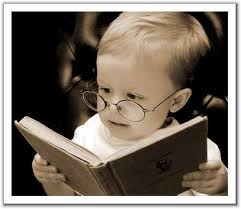
\includegraphics[scale=0.35]{gambar/child.png}
\end{wrapfigure}
Setiap hari kita berinteraksi dengan begitu banyak orang. Di keluarga, di tempat kerja, di sekelah, atau dimanapun kita akan membuat hubungan dengan begitu banyak orang. Tidak jarang, tiba-tiba timbul persoalan atau juga konflik dalam hubungan kita dengan orang lain. Tapi, itulah hidup! Namun, bagaimana kita menyikapi koflik tersebut?
Apakah kita percaya bahwa Tuhan bisa memakai orang - orang di sekitar kita, bahkan yang sedang berkonflik dengan kita, untuk membentuk karakter dalam hidup kita?

Jika kita ingin memaknai hidup dengan cara seperti itu, kita perlu 4 prinsip hidup berikut dalam berhubungan dengan orang lain:
\begin{enumerate}
\item Jagalah hati. Firman Tuhan berkata: ``Jagalah hatimu dengan segala kewaspadaan, karena dari situlah terpancar kehidupan.'' Ketika kita menerima kata - kata atau perlakuan yang menyakitkan, Jagalah Hati. Jika kita bisa menjaga kondisi hati kita untuk tidak mudah terpengaruh emosi dan tindakan orang lain, kita akan mampu melepaskan pengampunan dan lepas dari belenggu sakit hati.
\item Jagalah perkataan. Kita tidak hanya perlu memperhatikan apa yang kita ucapkan, tetapi juga cara mengucapkannya. Ada kalanya hanya karena salah ucap, atau nada suara dan ungkapan sinis bisa memancing sebuah pertengkaran. Hindarilah perkataan - perkataan yang tajam dan tidak perlu.
\item Jangan ungkit kegagalan masa lalu. Ingat, mungkin kita sedang bicara dengan orang yang perncah gagal di masa lalu. Daripada mengungkit-ungkit masa lalu yang bisa menimbulkan kesalahpagaman, lebih baik membicarakan hal-hal yang sekarang.
\item Jangan menunjukkan perkataan yang sombong. Tidak perlu memuji diri karena sebuah perbuatan yang pernah kita lakukan. Sikap rendah hati adalah kuncu dalam menjalin komunikasi yang positif. Belajarlah untuk bersuka cita ketika orang lain menerima pujian, sekalipun saat itu kita pun layak menerimanya.
\end{enumerate}

\begin{center}
\textbf{Belajarlah setiap hari untuk mendatangkan damai sejahtera bagi setiap orang.}\\
`` \ldots \textit{Sehingga kamu hidup sebagai orang - orang yang sopan di mata orang luar dan tidak bergantung pada mereka.} (1 Tesalonika 4 : 12)
\end{center}

\sumber{Kiriman Aditya Bimantara\\
dari ``Empat Prinsip Hidup.'' Renungan Harian Kita Maret 2010 \\  
http://www.renungan-harian-kita.blogspot.com.} 
\normalsize
\chap{Ketika Garam Kehilangan Asinnya}
\small
\begin{wrapfigure}{r}{3cm}
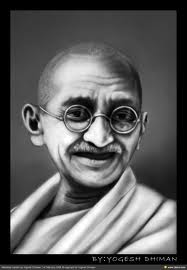
\includegraphics[scale=0.45]{gambar/gandhi.png}
\end{wrapfigure}
``Kamu adalah garam dunia, jika garam itu menjadi tawar, dengan apakah ia diasinkan? Tidak ada lagi gunanya selain dibuang dan diinjak orang'' (Mat. 5:13).
Mahadma Gandhi pernah sangat kecewa kepada orang Kristen di india karena sikap mereka yang sangat arogan dan suka membeda - bedakan. ``Aku bersimpati kepada ajaran Yesusmu, akan tetapi sangat muak dengan cara hidupmu'', ucap tokoh negeri Sungai Gangga yang dikenal seantero dunia ini. 

Mengapa banyak orang kecewa terhadap gereja?

Kecewa terhadap pengikut Kristus yang seharusnya menjadi batu lompatan untuk mengenal Kristus?

Mengapa mereka tidak dapat melanjutkan ketertarikan mereka kepada Kristus saat mereka melihat cara hidup orang-orang yang menamakan diri sebagai pengikut Kristus?

Pembaca Warta Iman terkasih, kali ini firman Tuhan mengingatkan kembali inti keberadaan kita di atas muka bumi ini. ``Kamu adalah garam dunia. Jika garam Kehilangan asinnya tidak ada gunanya lagi kecuali dibuang dan diinjak-injak orang'', demikian pesan Tuhan Yesus.

Pada zaman itu, garam yang dipakai untuk memasak menempel pada suatu media yang bisa berupa bunga karang atau lainnya. Setiap kali garam dipakai dimasukkan ke dalam tempat yang telah disediakan sebagai wadah memasak. Ketika garam yang menempel di bunga karang itu habis, maka media tersebut akan dibuang. Mengapa Demikian?? Karena manfaatnya telah tiada. Tinggal sisa-sisa yang tidak ada gunanya lagi!!!

Sebagai orang yang percaya kepada Tuhan Yesus. Seberapa besarkah tekad kita untuk menjadi sarana-Nya sehingga olehnya banyak orang yang datang kepada Dia? Sudahkah kita memahami rencan-Nya bagi dunia ini? Yakni agar segenap lutut berlutut dan mengaku bahwa Kristus adalah Tuhan bagi kemuliaan Allah Bapa!

\begin{center}
``Tuhan ajari aku agar mengerti maksudMu. Bimbing aku supaya berhasil 
menggarami dunia ini.''
\end{center}

\sumber{Kiriman Aditya Bimantara\\
dari ``Ketika Garam Kehilangan Asinnya'' Renungan Harian Kita Maret 2010 \\  
http://www.renungan-harian-kita.blogspot.com.} 
\normalsize

\chap{Warta Lingkungan}

\subsection*{APP}
Bulan Maret 2012 sudah masuk dalam masa Prapaskah. Sesuai dengan tradisi, setiap masa Prapaskah diadakan Aksi Puasa Pembangunan yang kegiatannya antara lain adalah ibadat APP di lingkungan. Untuk tahun ini Keuskupan Agung Semarang (KAS) menetapkan tema APP: \textit{Umat Katolik Sejati Harus Peduli dan Berbagi}. Dalam pelaksanaan di lingkungan St. Petrus, ibadat APP banyak diisi dengan \textit{sharing} yang mengacu pada buku panduan dari KAS.
Topik APP berawal dari baptis. Kapan kita dibaptis, kesan-kesan saat dibaptis, dan relevansinya dengan hidup menggereja dan bermasyarakat.

\subsection*{Misa pemberkatan rumah dan mitoni}
Bulan ini umat St. Petrus bertambah lagi dengan satu keluarga yang secara resmi bergabung sebagai warga lingkungan. Keluarga Bapak R. Mulyadi yang bertempat tinggal di Nanggulan, mengadakan misa syukur pemberkatan rumah dan sekaligus mitoni pada tanggal 22 Maret. Cicilia Nony Prayoga yang merupakan putri dari Bapak/Ibu Mulyadi menantikan kelahiran putranya bersama dengan suami tercinta
Bernadus Budhiprayoga.

Misa dipimpin oleh Rm. Albertus Purnomo, OFM yang merupakan kenalan baik keluarga R. Mulyadi saat masih di Jakarta. Dalam homilinya Romo menekankan bahwa Musa dapat melakukan tawar-menawar dengan Tuhan karena kedekatan Musa dengan Tuhan. Kenapa Musa dekat dengan Tuhan, karena Musa sering berdoa dan menaati perintah-Nya. Oleh karena itu kalau kita ingin dekat dengan Tuhan, maka rajin-rajinlah berdoa dan senantiasa menaati perintah-Nya.

\subsection*{Pendaftaran Krisma}
Telah diumumkan di gereja bahwa sakramen Krisma untuk paroki Marganingsih Kalasan akan dilangsungkan bulan September 2012. Calon penerima sakramen Krisma dapat mendaftarkan diri ke Ibu Munarti, Bapak Neo Suradi, atau kepada ketua lingkungan, dengan menyerahkan fotokopi surat baptis.

% SELECT day(`TglLahir`),
% concat(u1.`Baptis`,' ',u1.`Nama`) 
% FROM `umat` u1 WHERE month(TglLahir)=6 order by 1

%=========
% SELECT day(`TglNikah`),
% concat(u1.`Baptis`,' ',u1.`Nama`,' + ',u2.`Baptis`,' ',u2.`Nama`) 
% FROM `umat` u1 join kk on (u1.nokk=kk.id and u1.hubkel='KK')
%               join umat u2 on (u2.nokk=kk.id  and (u2.hubkel='istri' or u2.hubkel='isteri'))
% WHERE month(TglNikah)=1 order by 1

\section*{Yang berulang tahun kelahiran bulan ini}

\noindent{Semoga hari bahagia ini menguatkan imannya akan Dikau.}

\begin{longtable}{|c|l|} 
\hline
Tgl & Nama \\ \hline
\endhead1& Maria Rosary Sekar Seruni\\
5& Anna Maria Tri Henaningsih\\
6& Fransiscus Xaverius Sularto\\
7& Christina Sutarni\\
8& Marcellina Oktavia S. Padmini\\
11& Priscilla Oktiva Rossari\\
15& Yoseph Laba Atawolo\\
16& Ignatius Stanley Andi Pradana\\
18& Christina Sri Ning Hastuti\\
24& Margareta Maria Sri Pramuwati\\
25& Kristina Tri Tutwuri\\
\hline
\end{longtable}



\section*{Yang berulang tahun perkawinan  bulan ini}

Selamat ulang tahun perkawinan. Semoga keluarga-keluarga ini tumbuh menjadi keluarga Katolik yang sejati yang dibangun atas dasar iman dan kasih: kasih akan Dikau dan kasih antar semua anggota keluarga.

\begin{longtable}{|c|l|} 
\hline
Tgl & Keluarga \\ \hline
\endhead5& Nikolas Putut Andoko + Chatarina Krisyanti\\
6& Ignatius Luddy Indra Purnama + Anna Sri Wuryaningtyas\\
\hline
\end{longtable} 

\newpage
\chap{Kompendium Katekese Gereja Katolik}
\setcounter{kgkcounter}{29}
{\normalsize
\section*{KAMI PERCAYA}

\kgk{Mengapa iman itu tindakan pribadi dan sekaligus gerejawi?}
     Iman adalah tindakan pribadi sejauh menjadi jawaban bebas pribadi manusiawi kepada Allah yang mewahyukan Diri-Nya. Tetapi, sekaligus merupakan tindakan gerejawi yang mengungkapkan dirinya dalam pengakuan ``Kami percaya''.
Kenyataannya, Gerejalah yang percaya, dan dengan rahmat Roh Kudus, Gereja
mendahului, memunculkan, dan memperkembangkan iman setiap orang Kristen.
Karena alasan inilah Gereja adalah Bunda dan Guru.

\kgk{Mengapa rumusan iman itu penting?}
     Rumusan iman itu penting karena dengannya orang beriman dapat mengungkapkan, menghayati, merayakan, dan saling berbagi kebenaran-kebenaran iman
bersama dengan orang beriman lainnya melalui satu bahasa yang sama.

\kgk{Mengapa iman Gereja itu hanya satu?}
       Gereja, walaupun terdiri dari banyak orang dari macam-macam bahasa,            budaya, dan ritus, mengakui satu iman dalam kesatuan suara; iman yang diterima        dari satu Allah dan diwariskan oleh satu Tradisi Apostolik. Gereja hanya mengakui
satu Allah, Bapa, Putra, dan Roh Kudus, dan menunjuk pada satu jalan keselamatan.
Karena itu, kita percaya dengan satu hati dan satu jiwa semua yang terdapat dalam
Sabda Allah, diwariskan langsung atau ditulis, dan diakui oleh Gereja sebagai wahyu
ilahi.

\kgk{Apa simbol-simbol iman itu?}
     Simbol-simbol iman adalah rumusan-rumusan yang diformulasikan, disebut 
juga ”pengakuan iman” atau ”syahadat”. Sejak awal mula berdirinya, Gereja merumuskan pengakuan iman ini secara sintetis dan mewariskannya dalam bahasa
yang normatif dan umum bagi semua umat beriman.


\flushright{(\dots \emph{bersambung} \dots)}
}
\end{document}